\chapter{Lec 02 - Problem Solving Agent}
\section{Solving Problems by Searching}
We'll describe one kind of \textbf{goal-based} agent called a problem-solving agent. Our discussion of problem solving begins with precise definitions of \textbf{problems} and their \textbf{solutions} and give several examples to illustrate these definitions. We then describe several
general-purpose search algorithms that can be used to solve these problems. We will see several \textbf{uninformed} search algorithms, algorithms that are given no information about the problem other than its definition. Let's start with an example:\newline\newline
Imagine an agent in the city of Arad, Romania, enjoying a touring holiday. Now, suppose the agent has a nonrefundable ticket to fly out of Bucharest the following day. In that case, it makes sense for the agent to adopt the \textbf{goal} of getting to Bucharest by driving across various cities. Therefore, the \textbf{problem formulation} can be defined as follows:
\begin{itemize}
    \item Formulate goal: be in Bucharest
    \item Formulate problems:
    \begin{itemize}
        \item states: various cities
        \item actions: drive between cities
    \end{itemize}
    \item Solution: sequence of cities; e.g. Arad, Sibiu, Fagaras, Bucharest
\end{itemize}
\begin{center}
    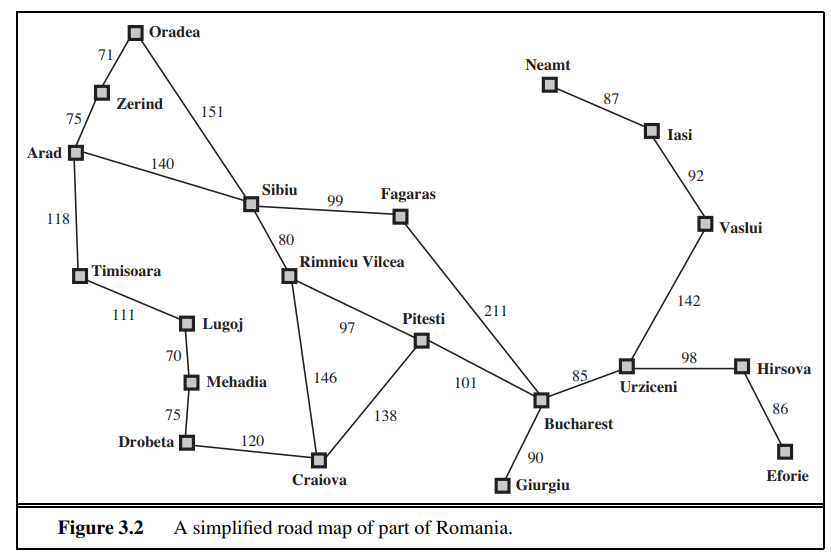
\includegraphics[scale=0.8]{images/Romania.png}
\end{center}
We assume that the environment is \textbf{observable}, so the agent always knows the current state. For the agent driving in Romania, it’s reasonable to suppose that each city on the map has a sign indicating its presence to arriving drivers. We also assume the environment is \textbf{discrete}, so at any given state there are only finitely many actions to choose from. This is true for navigating in Romania because each city is connected to a small number of other cities. We will assume the environment is \textbf{known}, so the agent knows which states are reached by each action. (Having an accurate map suffices to meet this condition for navigation problems.) Finally, we assume that the environment is \textbf{deterministic}, so each action has exactly one outcome.\newline\newline
The process of looking for a sequence of actions that reaches the goal is called \textbf{search}. A search algorithm takes a problem as input and returns a \textbf{solution} in the form of an action sequence.
\begin{center}
    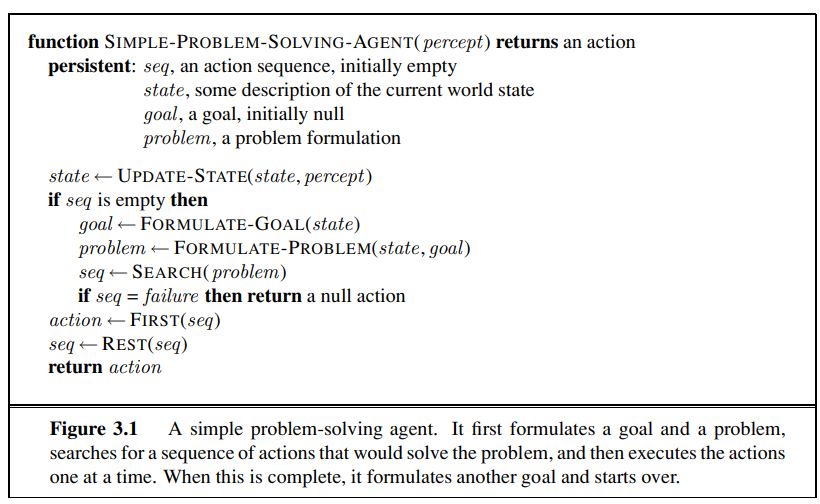
\includegraphics[scale=0.8]{images/problem-solving agent.png}
\end{center}
A problem can be defined formally by four components:
\begin{itemize}
    \item The \textbf{initial state} that the agent starts in. For example, the initial state for our agent in Romania might be described as \textit{In(Arad)}.

    \item A description of what each action does; the formal name for this is the \textbf{transition model}. We also use the term \textbf{successor} to refer to any state reachable from a given state by a single action. This can be described by a set $E(x)$ of action-state pairs, e.g. $E(In(Arad)) = \{<Arad \rightarrow Zerind, Zerind>, ...\}$. An alternative formulation for the successor function can be the actions that can be performed in a given state.

    \item The \textbf{goal test}, which determines whether a given state is a goal state. The goal can be explicit, e.g. the singleton set \footnote{There can be multiple goal states} $\{In(Bucharest)\}$, or implicit, an abstract property rather than an explicitly enumerated set of states.

    \item A \textbf{path cost} function that assigns a numeric cost to each path. The problem-solving agent chooses a cost function that reflects its own performance measure. For the agent trying to get to Bucharest, time is of the essence, so the cost of a path might be its length in kilometers. The \textbf{step cost} of taking action $a$ in state $s$ to reach state $s'$ is denoted by $c(s, a, s')$, assumed to be $\geq 0$.
\end{itemize}
The preceding elements define a problem and can be gathered into a single data structure that is given as input to a problem-solving algorithm. A solution to a problem is an action sequence that leads from the initial state to a goal state. Solution quality is measured by the path cost function, and an \textbf{optimal solution} has the lowest path cost among all solutions.

\section{Selecting a State Space}
Real world is absurdly complex. Compare the simple state description we have chosen, $In(Arad)$, to an actual crosscountry trip, where the state of the world includes so many things: the traveling companions, the current radio program, the scenery out of the window, the proximity of law enforcement officers, etc. All these considerations are left out of our state descriptions because they are irrelevant to the problem of finding a route to Bucharest. The process of removing detail from a representation is called \textbf{abstraction}.
\newline\newline
In addition to abstracting the state description, we must abstract the actions themselves.\newline\newline
Now consider a solution to the abstract problem: for example, the path from Arad to Sibiu to Rimnicu Vilcea to Pitesti to Bucharest. This abstract solution corresponds to a large number of more detailed paths.
\newline\newline
The choice of a good abstraction thus involves removing as much detail as possible while retaining validity and ensuring that the abstract actions are easy to carry out.

\section{Searching for Solutions}
A solution is an action sequence, so search algorithms work by considering various possible action sequences. The possible action sequences starting at the initial state form a \textbf{search tree} with the initial state at the root; the branches are actions and the \textbf{nodes} correspond to states in the \textbf{state space} of the problem.
\begin{center}
    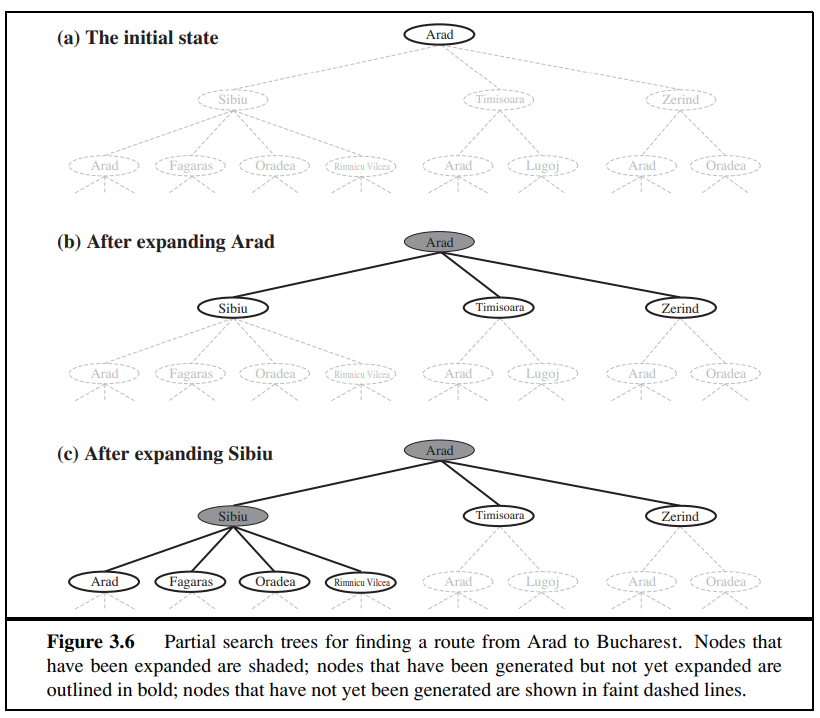
\includegraphics[scale=0.8]{images/search tree.png}
\end{center}
We start from the root and, at each step, we need to check whether we reached the goal state. Then, we need to consider taking various actions. We do this by \textbf{expanding} the current state, that is, applying each legal action to the current state, thereby \textbf{generating} a new set of states. In the case of the figure above, we add three branches from the parent node $In(Arad)$ leading to three new child nodes: $In(Sibiu)$, $In(Timisoara)$, and $In(Zerind)$. Now we must choose which of these three possibilities to consider further.\newline\newline
This is the essence of search, following up one option now and putting the others aside for later. The set of all leaf nodes available for expansion at any given point is called the \textbf{frontier}. The process of expanding nodes on the frontier continues until either a solution is found or there are no more states to expand.
\begin{center}
    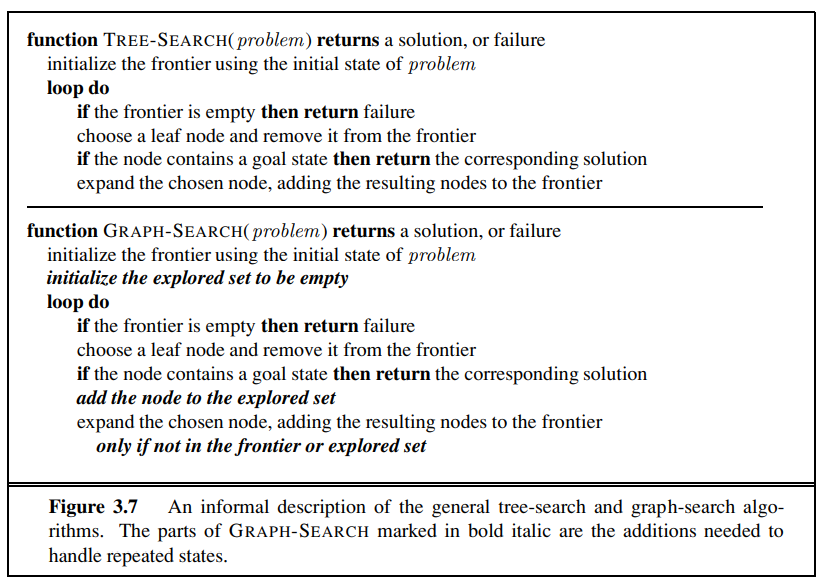
\includegraphics[scale=0.8]{images/tree search2.png}
\end{center}
Search algorithms all share the basic structure above; they vary primarily according to how they choose which state to expand next, the so-called search strategy.\newline\newline
In the figure representing the search tree of the \textit{driving through Romania} problem we can notice that it includes the path from Arad to Sibiu and back to Arad again. We say that $In(Arad)$ is a \textbf{repeated state} in the search tree, generated in this case by a \textbf{loopy path}.\newline\newline
The way to avoid exploring redundant paths is to remember where one has been. To do this, we augment the TREE-SEARCH algorithm with a data structure called the \textbf{explored set} (also known as the closed list), which remembers every expanded node. Newly generated nodes
that match previously generated nodes can be discarded instead of being added to the frontier. This new algorithm is called GRAPH-SEARCH.\newline\newline
Clearly, the search tree constructed by the GRAPH-SEARCH algorithm contains at most one copy of each state, so we can think of it as growing a tree directly on the state-space graph. Furthermore, the frontier \textbf{separates} the state-space graph into the explored region and the unexplored region, so that every path from the initial state to an unexplored state has to pass through a state in the frontier.\newline\newline
Up to now, we have not been very careful to distinguish between nodes and states, but in writing detailed algorithms it’s important to make that distinction. A node is a bookkeeping data structure used to represent the search tree. It includes \textit{parent, children, depth, path cost}. A state corresponds to a configuration of the
world. Thus, nodes are on particular paths whereas states are not. Furthermore, two different nodes can contain the same world state if that state is generated via two different search paths.\newline\newline
Now that we have nodes, we need somewhere to put them. The frontier needs to be stored in such a way that the search algorithm can easily choose the next node to expand according to its preferred strategy. The appropriate data structure for this is a \textbf{queue}.

\section{Uninformed Search Strategies}
Uniformed Search Strategies include the following:
\begin{itemize}
    \item \textbf{Breadth-first search:} Breadth-first search is a simple strategy in which the root node is expanded first, then all the successors of the root node are expanded next, then their successors, and so on. In general, all the nodes are expanded at a given depth in the search tree before any nodes at the next level are expanded. The frontier is implemented using a FIFO queue.

    \item \textbf{Uniform-cost search:} The idea is to expand least-cost unexpanded node. This is done by storing the frontier as a priority queue ordered by path cost.

    \item \textbf{Depth-first search:} Depth-first search always expands the deepest node in the current frontier of the search tree. the frontier is implemented as a LIFO queue.

    \item \textbf{Iterative deepening depth-first search:} Iterative deepening search (or iterative deepening depth-first search) which repeatedly applies depth first search limiting the depth of the tree. It does this by gradually increasing the limit, first 0, then 1, then 2, and so on, until a goal is found.

    \item \textbf{Bidirectional search:} The idea behind bidirectional search is to run two simultaneous searches—one forward from the initial state and the other backward from the goal—hoping that the two searches meet in the middle.

\end{itemize}
We can evaluate an algorithm’s performance in four ways:
\begin{itemize}
    \item \textbf{Completeness:} Is the algorithm guaranteed to find a solution when there is one?

    \item \textbf{Optimality:} Does the strategy find the optimal solution in terms of cost?

    \item \textbf{Time complexity:} How long does it take to find a solution?

    \item \textbf{Space complexity:} How much memory is needed to perform the search?
\end{itemize}
The evaluation of the previously presented strategies is the following:
\begin{center}
    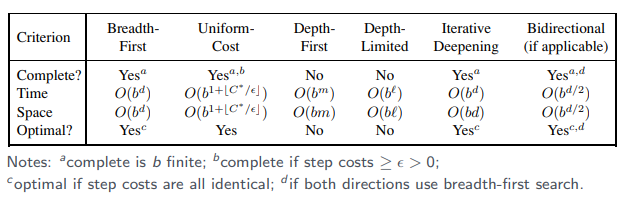
\includegraphics[]{images/evaluation.png}
\end{center}
where:
\begin{itemize}
    \item $b$ is the branching factor (how many successor a node has)

    \item $d$ is the depth of the shallowest solution

    \item $m$ is the maximum depth of the search tree

    \item $l$ is the depth limit
\end{itemize}
We can easily see that \textbf{Breadth-first search} is complete; if the shallowest goal node is at some finite depth $d$, breadth-first search will eventually find it after generating all shallower nodes. Note that as soon as a goal node is generated, we know it is the shallowest goal node because all shallower nodes must have been generated already
and failed the goal test. However, the shallowest goal node is not necessarily the optimal one. Furthermore, every node generated remains in
memory, making the space complexity $O(b^d)$\newline\newline
On the other hand, \textbf{Uniform-cost search} is optimal in general. First, we observe that whenever uniform-cost search selects a node $n$ for expansion, the optimal path to that node has been found. Then,
because step costs are non-negative, paths never get shorter as nodes are added.\newline\newline
The properties of \textbf{depth-first search} depend strongly on whether the graph-search or tree-search version is used. The graph-search version, which avoids repeated states and redundant paths, is complete in finite state spaces because it will eventually expand every node. The tree-search version, on the other hand, is not complete (it may get stuck in a loop). The time complexity of depth-first tree search is $O(b^m)$. Note that $m$ itself can be much larger than $d$. So far, depth-first search seems to have no clear advantage over breadth-first search, so why do we include it? The reason is the space complexity. For a graph search, there is no advantage, but a depth-first tree search needs to store only a single path from the root to a leaf node, along with the remaining unexpanded sibling nodes for each node on the
path. Once a node has been expanded, it can be removed from memory as soon as all its descendants have been fully explored.\newline\newline
We can combine the completeness of BFS and the space saving of DFS with the \textbf{Iterative deepening search}. This strategy may seem wasteful because states are generated multiple times. It turns out this is not too costly. The reason is that in a search tree with the same (or nearly the same) branching factor at each level, most of the nodes are in the bottom level, so it does not matter much that the upper levels are generated multiple times.\newline\newline


